%%%%%%%%%%%%%%%%%%%%%%%%%%%%%%%%%%%%%%%%%%%%%%%%%%%%%%%%%%%%%%%%%%%%%%%%%%%%%%%%
%%%%%%%%%%%%%%%%%%%%%%%%%%%%%%%%%%%%%%%%%%%%%%%%%%%%%%%%%%%%%%%%%%%%%%%%%%%%%%%%
\exercice{Étude et conception de correcteurs AP, PI et PID\difficile}
%%%%%%%%%%%%%%%%%%%%%%%%%%%%%%%%%%%%%%%%%%%%%%%%%%%%%%%%%%%%%%%%%%%%%%%%%%%%%%%%
%%%%%%%%%%%%%%%%%%%%%%%%%%%%%%%%%%%%%%%%%%%%%%%%%%%%%%%%%%%%%%%%%%%%%%%%%%%%%%%%
%%%%%%%%%%%%%%%%%%%%%%%%%%%%%%%%%%%%%%%%%%%%%%%%%%%%%%%%%%%%%%%%%%%%%%%%%%%%%%%%
%%%%%%%%%%%%%%%%%%%%%%%%%%%%%%%%%%%%%%%%%%%%%%%%%%%%%%%%%%%%%%%%%%%%%%%%%%%%%%%%
\subsection*{Caractérisation du système non corrigée}
%%%%%%%%%%%%%%%%%%%%%%%%%%%%%%%%%%%%%%%%%%%%%%%%%%%%%%%%%%%%%%%%%%%%%%%%%%%%%%%%
%%%%%%%%%%%%%%%%%%%%%%%%%%%%%%%%%%%%%%%%%%%%%%%%%%%%%%%%%%%%%%%%%%%%%%%%%%%%%%%%
%Q1
%%%%%%%%%%%%%%%%%%%%%%%%%%%%%%%%%%%%%%%%%%%%%%%%%%%%%%%%%%%%%%%%%%%%%%%%%%%%%%%%
\question{\textbf{Tracer le diagramme de Bode de la boucle ouverte 
          non corrigée}}
%%%%%%%%%%%%%%%%%%%%%%%%%%%%%%%%%%%%%%%%%%%%%%%%%%%%%%%%%%%%%%%%%%%%%%%%%%%%%%%%
La fonction de transfert en boucle ouverte non corrigée $H(p)$ est donnée par:
\[
    H(p)=\dfrac{5p+10}{p^3+3p^2+4p+2}
\]
Le programme Scilab ci-dessous permet de tracer le diagramme de Bode pour cette
fonction de transfert.
%-------------------------------------------------------------------------------
\inputminted{scilab}{codes/scilab/code_q1_chap_correction.sce}
%-------------------------------------------------------------------------------
%-------------------------------------------------------------------------------
\begin{figure}
    \centering
    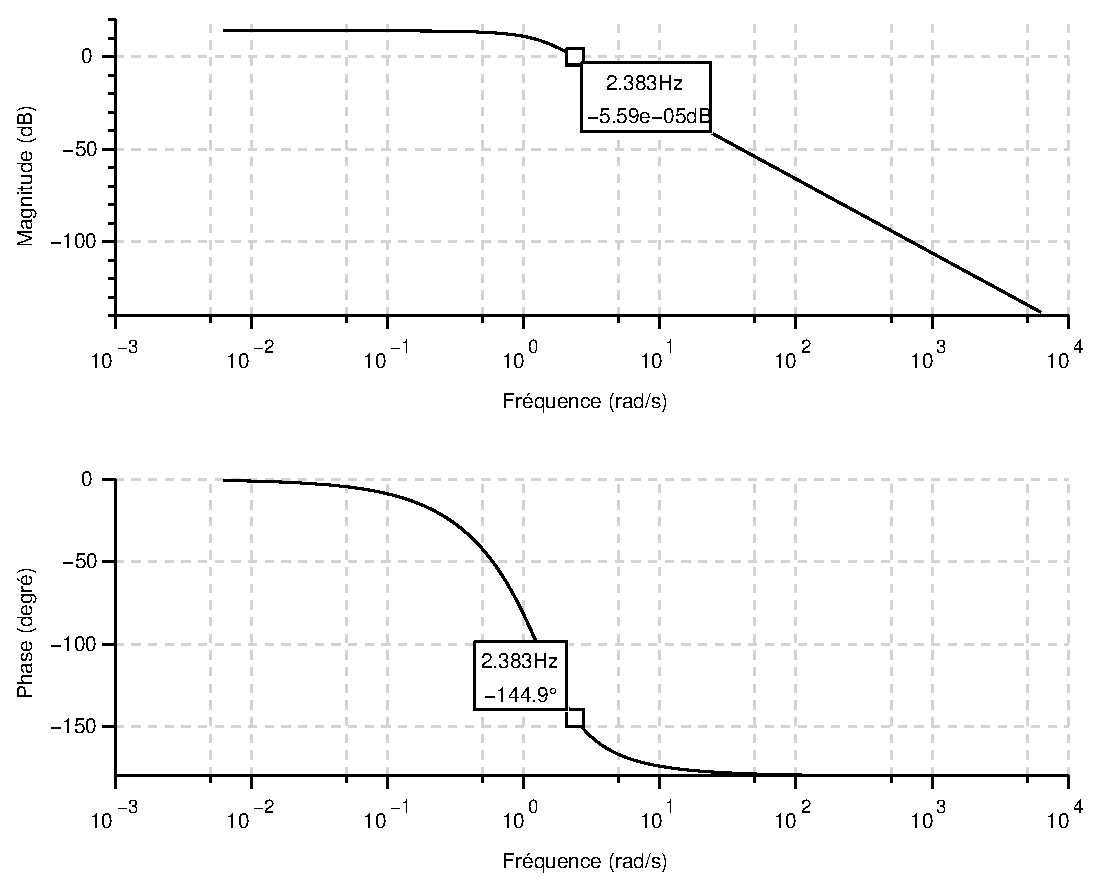
\includegraphics[width=0.75\textwidth]{bode_BONC.eps}
    \caption{Diagramme de Bode de la boucle ouverte non corrigée. 
             On a représenté le gain et la phase à la pulsation de coupure 
             $\omega_{\SI{0}{\dB}}$ du système non corrigée.}
\end{figure}
%-------------------------------------------------------------------------------
Comme attendu le déphasage est nulle à basse fréquence (BF) et de 
\SI{-180}{\degreeSI} à haute fréquence (HF) (degré 1 au numérateur et 
degré 3 au dénominateur). De même la pente du gain est nulle à BF et 
de \SI{-40}{\dB\per\dec}.
%Q2
%%%%%%%%%%%%%%%%%%%%%%%%%%%%%%%%%%%%%%%%%%%%%%%%%%%%%%%%%%%%%%%%%%%%%%%%%%%%%%%%
\question{\textbf{Déterminer la pulsation $\omega_{\SI{0}{\dB}}$, telle que le 
          gain de la fonction de transfert en boucle ouverte soit 
          égale à \SI{0}{\dB}}}
%%%%%%%%%%%%%%%%%%%%%%%%%%%%%%%%%%%%%%%%%%%%%%%%%%%%%%%%%%%%%%%%%%%%%%%%%%%%%%%%
D'après le diagramme de Bode précédent, on mesure graphiquement une pulsation
$\omega_{\SI{0}{\dB}}=\SI{2.383}{\radian\per\second}$.
Par le calcul, on déterminer cette valeur comme la pulsation qui donne un 
module de la fonction de transfert en boucle ouverte complexe égal à 1.
On cherche donc $\omega$ tel que :
%-------------------------------------------------------------------------------
\begin{align*}
    |H(j\omega)|=1 &\iff \\
    \dfrac{|10+j5\omega|}{|(2-3\omega^2)+\jw(4-\omega^2)|}=1 &\iff \\
    \dfrac{100+25\omega^2}{\omega^6+\omega^4+4\omega^2+4}=1 &\iff \\
    \omega^6+\omega^4-21\omega^2-96=0
\end{align*}
%-------------------------------------------------------------------------------
Pour résoudre cette équation, on pourrait utiliser l'instruction Scilab 
suivante :
%-------------------------------------------------------------------------------
\inputminted{scilab}{codes/scilab/code_q2_1_chap_correction.sce}
%-------------------------------------------------------------------------------
La solution réelle et positive de cette équation est bien la pulsation obtenue
graphiquement.

Il est possible de vérifier ceci en calculant le module et la phase de la 
fonction de transfert en boucle ouverte non corrigée à cette pulsation. 
(En utilisant les fonctions Scilab \texttt{repfreq} et \texttt{dbphi}). 
%-------------------------------------------------------------------------------
\inputminted{scilab}{codes/scilab/code_q2_2_chap_correction.sce}
%-------------------------------------------------------------------------------

%Q3
%%%%%%%%%%%%%%%%%%%%%%%%%%%%%%%%%%%%%%%%%%%%%%%%%%%%%%%%%%%%%%%%%%%%%%%%%%%%%%%%
\question{\textbf{Déterminer si le système est stable en boucle fermée par la 
          méthode de votre choix. Si oui, déterminer la marge de 
          phase $M_\phi$}}
%%%%%%%%%%%%%%%%%%%%%%%%%%%%%%%%%%%%%%%%%%%%%%%%%%%%%%%%%%%%%%%%%%%%%%%%%%%%%%%%
D'après le diagramme de Bode de la boucle ouverte, le système est stable 
en boucle fermée par le critère de Nyquist. On peut également le vérifier 
en déterminant les pôles de la fonction de transfert en boucle fermée.
\[
    H_{BF}=\dfrac{5p+10}{p^3+3p^2+9p+12}
\]
%-------------------------------------------------------------------------------
\inputminted{scilab}{codes/scilab/code_q3_chap_correction.sce}
%-------------------------------------------------------------------------------
Les pôles sont tous à partie réelle négative ce qui confirme la conclusion 
précédente. Le critère pourrait également être appliqué.
%Q4
%%%%%%%%%%%%%%%%%%%%%%%%%%%%%%%%%%%%%%%%%%%%%%%%%%%%%%%%%%%%%%%%%%%%%%%%%%%%%%%%
\question{\textbf{Tracer la réponse indicielle de la boucle fermée et 
          déterminer la valeur finale de la boucle fermée. On pourra donner
          certaines grandeurs caractérisant sa rapidité, son dépassement}}
%%%%%%%%%%%%%%%%%%%%%%%%%%%%%%%%%%%%%%%%%%%%%%%%%%%%%%%%%%%%%%%%%%%%%%%%%%%%%%%%
%-------------------------------------------------------------------------------
\inputminted{scilab}{codes/scilab/code_q4_chap_correction.sce}
%-------------------------------------------------------------------------------
\begin{figure}
    \centering
    \tikzsetnextfilename
    {reponse_indicielle_non_corrige-exercices_corriges-chap_correction-ext}
    \begin{tikzpicture}
    \begin{axis}
    [
        axis x line=center,
        axis y line=center,
        xlabel={$t$},
        ylabel={$s(t)$},
        x label style ={below},
        y label style ={left},
        xtick={2.5,5,7.5,10},
        xticklabels={2.5,5,7.5},
        ytick={0,0.25,0.5,0.75,1.0,1.25,1.5},
        yticklabels={0,,0.5,,1.0},
        grid=both,
        ymin=0,ymax=1.2,
    ]
    \addplot[mark=none,col4,ultra thick] 
            table {scilab/step_response_hbf_NC.dat};
    \addplot[col4,dashed,domain=0:10] {0.83333*0.95};
    \addplot[col4,dashed,domain=0:10] {0.83333*1.05};
    \end{axis}
\end{tikzpicture}

    \caption{Réponse indicielle du système en boucle fermée non corrigé}
\end{figure}
%-------------------------------------------------------------------------------
La valeur finale est graphiquement égale à 0.83 .
Par le calcul il suffit d'appliquer le théorème de la valeur finale:
\[
    \lim\limits_{p\to0} pS(p)=
    \lim\limits_{p\to0} pH_{BF}(p)E(p)=
    \lim\limits_{p\to0} H_{BF}(p)=\dfrac{5}{6}\sim0.833
\]
pour $E(p)=\dfrac{1}{p}$.
Le temps de réponse à 5\% est de l'ordre de \SI{5}{\second} et le premier 
dépassement de 40\%.
%%%%%%%%%%%%%%%%%%%%%%%%%%%%%%%%%%%%%%%%%%%%%%%%%%%%%%%%%%%%%%%%%%%%%%%%%%%%%%%%
%%%%%%%%%%%%%%%%%%%%%%%%%%%%%%%%%%%%%%%%%%%%%%%%%%%%%%%%%%%%%%%%%%%%%%%%%%%%%%%%
\subsection*{Régulation du correcteur à avance de phase}
%%%%%%%%%%%%%%%%%%%%%%%%%%%%%%%%%%%%%%%%%%%%%%%%%%%%%%%%%%%%%%%%%%%%%%%%%%%%%%%%
%%%%%%%%%%%%%%%%%%%%%%%%%%%%%%%%%%%%%%%%%%%%%%%%%%%%%%%%%%%%%%%%%%%%%%%%%%%%%%%%
On souhaite corriger le système en rapidité et en robustesse (augmenter la 
marge de stabilité). Pour augmenter la bande passante en boucle fermée, on 
décide de fixer la pulsation de coupure $\omega_0$ à 
\SI{4}{\radian\per\second} et on cherche à obtenir parallèlement une marge 
de phase $M_\phi$ de \SI{60}{\degreeSI}.

%Q5
%%%%%%%%%%%%%%%%%%%%%%%%%%%%%%%%%%%%%%%%%%%%%%%%%%%%%%%%%%%%%%%%%%%%%%%%%%%%%%%%
\question{\textbf{À partir du diagramme de Bode de la boucle ouverte 
          non corrigée, déterminer la phase $\phi_d$ et le gain $G_d$ devant 
          être apportés par le correcteur à avance de phase à la 
          pulsation de coupure que l'on s'est donnée.}}
%%%%%%%%%%%%%%%%%%%%%%%%%%%%%%%%%%%%%%%%%%%%%%%%%%%%%%%%%%%%%%%%%%%%%%%%%%%%%%%%
Le déphasage apporté par le système en boucle ouverte corrigée est donnée
par l'argument de la fonction de transfert complexe en  $\omega_0$. Soit
encore, 
\[
    \arg{\left(C_{PI}H(j\omega_0)\right)} = \phi_d + \arg{H(j\omega_0)}
\]
où $\phi_d$ est le déphasage apporté par le correcteur seul.
Pour une marge de phase souhaité de $M_\phi$. On cherche donc $\phi_d$
\[
    \phi_d=\SI{-180}{\degreeSI}+M_\phi-\arg{H(j\omega_0)}
\]
\[
    \phi_d=\SI{-120}{\degreeSI}-\arg{H(j\omega_0)}
\]
où $\arg{H(j\omega_0)}$ est le déphasage de la boucle ouverte non corrigée à 
la pulsation $\omega_0)$ (que l'on obtient graphiquement sur le diagramme de 
Bode.)
%-------------------------------------------------------------------------------
\begin{figure}
    \centering
    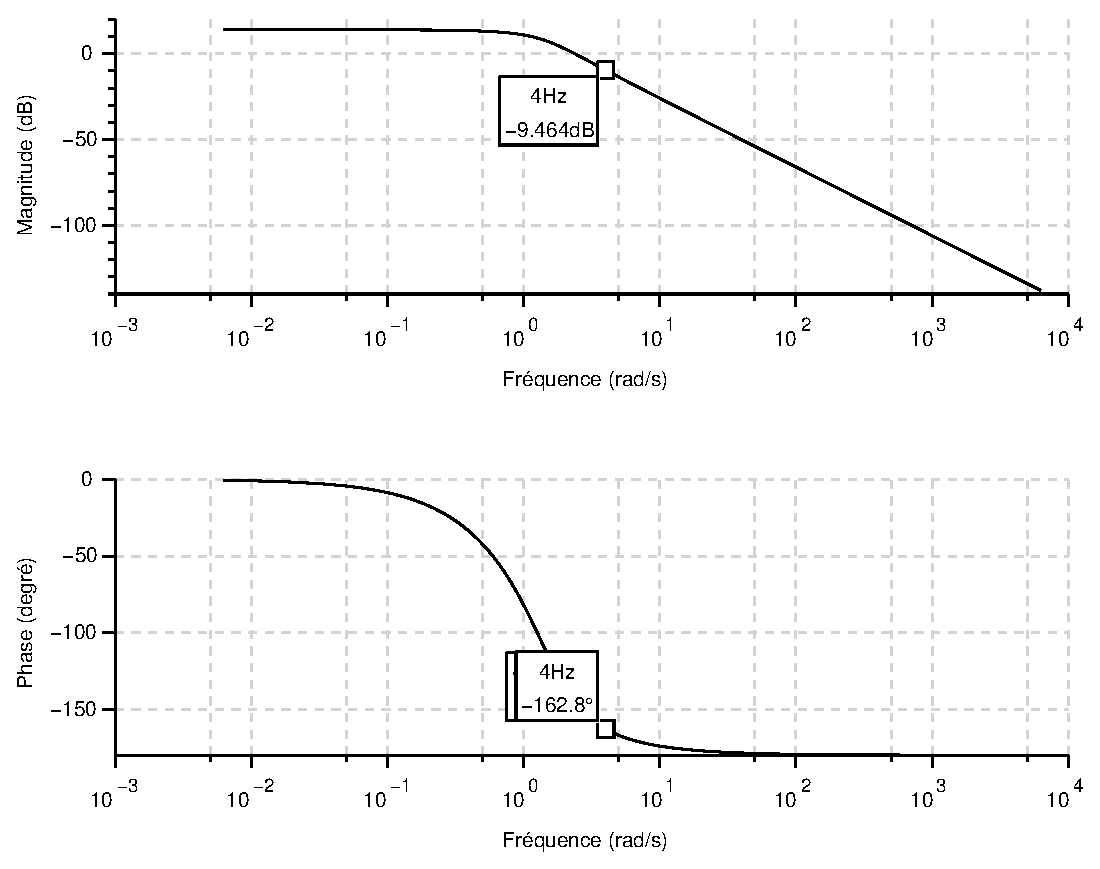
\includegraphics[width=0.75\textwidth]{bode_BONC_2.eps}
    \caption{Diagramme de Bode de la boucle ouverte non corrigée
             On a représenté le gain et la phase à la pulsation de coupure 
             $\omega_0=\SI{4}{\radian\per\second}$}
\end{figure}
%-------------------------------------------------------------------------------
On mesure $\arg{H(j\omega_0)}=\SI{-162.8}{\degreeSI}$ :
\[
    \phi_d=\SI{42.8}{\degreeSI}
\]
\[
    G_d=\SI{9.46}{\dB}=10^{9.46/20}=2.97
\]
%Q6
%%%%%%%%%%%%%%%%%%%%%%%%%%%%%%%%%%%%%%%%%%%%%%%%%%%%%%%%%%%%%%%%%%%%%%%%%%%%%%%%
\question{\textbf{À partir des relations suivantes, déterminer les paramètres 
$(\alpha,\tau_d,K_d)$ du correcteur à avance de phase}}
%%%%%%%%%%%%%%%%%%%%%%%%%%%%%%%%%%%%%%%%%%%%%%%%%%%%%%%%%%%%%%%%%%%%%%%%%%%%%%%%
On a alors :
%-------------------------------------------------------------------------------
\begin{align*}
    \alpha&=\dfrac{1+\sin\phi_d}{1-\sin\phi_d}=5.239 \\
    \tau_d&=\dfrac{1}{\omega_0\sqrt\alpha}=\SI{0.109}{\second}\\
       K_d&=\dfrac{G_d}{\sqrt\alpha}=1.298
\end{align*}
%-------------------------------------------------------------------------------
%Q7
%%%%%%%%%%%%%%%%%%%%%%%%%%%%%%%%%%%%%%%%%%%%%%%%%%%%%%%%%%%%%%%%%%%%%%%%%%%%%%%%
\question{\textbf{Donner la forme numérique de la fonction de transfert du 
          correcteur à avance de phase}}
%%%%%%%%%%%%%%%%%%%%%%%%%%%%%%%%%%%%%%%%%%%%%%%%%%%%%%%%%%%%%%%%%%%%%%%%%%%%%%%%
\[
C_{AP}(p)=\dfrac{1.298 + 0.743p } {1 + 0.109p}
\]
%Q8
%%%%%%%%%%%%%%%%%%%%%%%%%%%%%%%%%%%%%%%%%%%%%%%%%%%%%%%%%%%%%%%%%%%%%%%%%%%%%%%%
\question{\textbf{Tracer le diagramme de Bode de la boucle ouverte corrigée par 
          ce correcteur}}
%%%%%%%%%%%%%%%%%%%%%%%%%%%%%%%%%%%%%%%%%%%%%%%%%%%%%%%%%%%%%%%%%%%%%%%%%%%%%%%%
Les instructions Scilab ci-dessous permettent de tracer le diagramme 
de Bode de la boucle ouverte corrigée par un correcteur à avance de phase.
%-------------------------------------------------------------------------------
\inputminted{scilab}{codes/scilab/code_q8_chap_correction.sce}
%-------------------------------------------------------------------------------
%-------------------------------------------------------------------------------
\begin{figure}
    \centering
    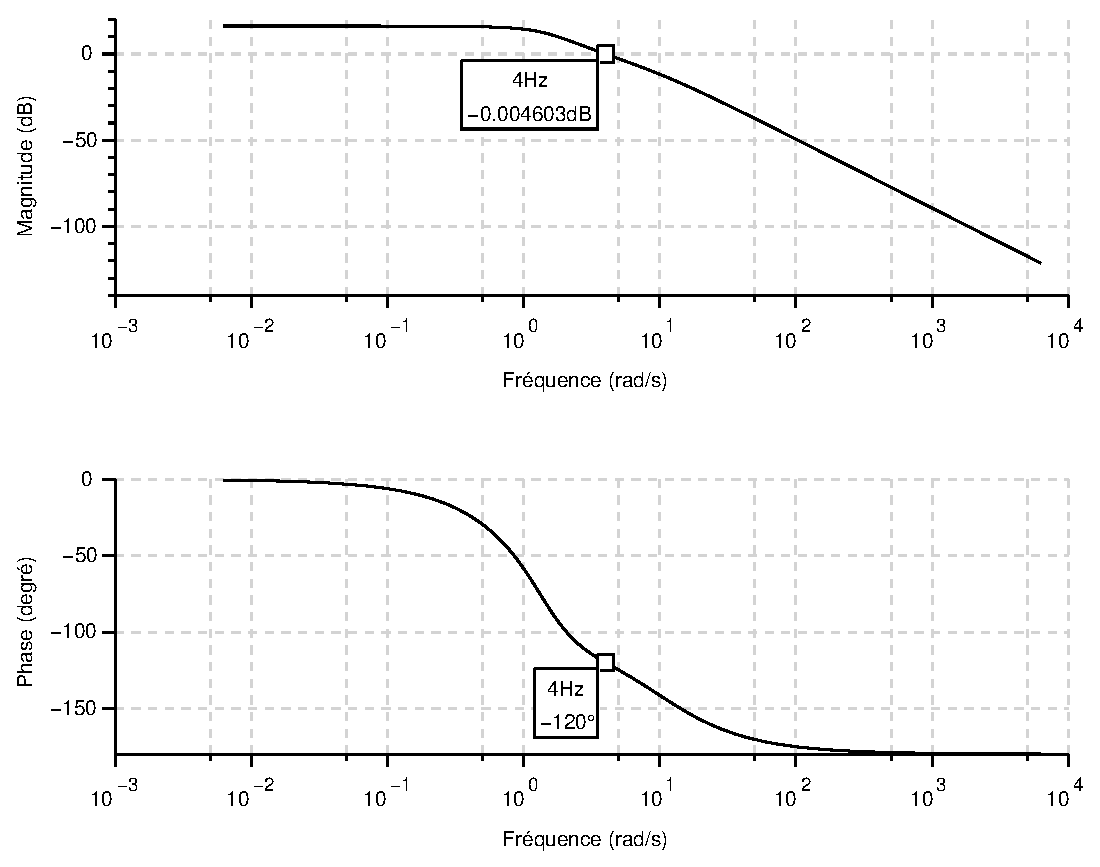
\includegraphics[width=0.75\textwidth]{bode_BOCAP.eps}
    \caption{Diagramme de Bode de la boucle ouverte corrigée par le correcteur
    à avance de phase}
\end{figure}
%-------------------------------------------------------------------------------
On vérifie bien que la marge de phase $M_\phi$ est égale à \SI{60}{\degreeSI}
à la pulsation de coupure de $\omega_0=\SI{4}{\radian\per\second}$.
%%%%%%%%%%%%%%%%%%%%%%%%%%%%%%%%%%%%%%%%%%%%%%%%%%%%%%%%%%%%%%%%%%%%%%%%%%%%%%%%
%%%%%%%%%%%%%%%%%%%%%%%%%%%%%%%%%%%%%%%%%%%%%%%%%%%%%%%%%%%%%%%%%%%%%%%%%%%%%%%%
\subsection*{Régulation du correcteur PI}
%%%%%%%%%%%%%%%%%%%%%%%%%%%%%%%%%%%%%%%%%%%%%%%%%%%%%%%%%%%%%%%%%%%%%%%%%%%%%%%%
%%%%%%%%%%%%%%%%%%%%%%%%%%%%%%%%%%%%%%%%%%%%%%%%%%%%%%%%%%%%%%%%%%%%%%%%%%%%%%%%
On souhaite maintenant rendre le système précis à l'aide de l'effet intégral
Cependant, on veut également garantir de nouveau une marge de phase $M_\phi$ de 
\SI{60}{\degree}. Pour maintenir le système stable, il faut donc centrer le 
correcteur PI à une pulsation $\omega_0<\omega_{\SI{0}{\dB}}$
%Q9
%%%%%%%%%%%%%%%%%%%%%%%%%%%%%%%%%%%%%%%%%%%%%%%%%%%%%%%%%%%%%%%%%%%%%%%%%%%%%%%%
\question{\textbf{Déterminer l'intervalle des pulsations pour laquelle 
          la marge de stabilité $M_\phi$ de \SI{60}{\degree} 
          est accessible}}
%%%%%%%%%%%%%%%%%%%%%%%%%%%%%%%%%%%%%%%%%%%%%%%%%%%%%%%%%%%%%%%%%%%%%%%%%%%%%%%%
Le déphasage apporté par le correcteur PI étant compris entre 
$\SI{-90}{\degree}$ et $\SI{0}{\degree}$, le déphasage du système 
corrigé ne peut présenter une marge de phase de $\SI{60}{\degree}$ que pour 
un certain intervalle de pulsations. En effet, puisque
\[
    \arg{H(j\omega_0)}=\SI{-180}{\degreeSI}+M_\phi-\phi_i,
\]
où $\arg{H(j\omega_0)}$ est le déphasage de la boucle ouverte non 
corrigé à la pulsation $\omega_0$ et $\phi_i$ le déphasage du 
correcteur tel que $\SI{-90}{\degreeSI}<\phi_i<\SI{0}{\degree}$. 
L'argument $\arg{H(j\omega_0)}$ est donc contraint par les 
bornes de $\phi_i$ :
\[
    \SI{-180}{\degreeSI}+M_\phi<\arg{H(j\omega_0)}<\SI{-90}{\degreeSI}+M_\phi
\]
soit pour $M_\phi=\SI{60}{\degreeSI}$
\[
    \SI{-120}{\degreeSI}<\arg{H(j\omega_0)}<\SI{-30}{\degreeSI}
\]
On peut relever sur le diagramme de Bode de la boucle ouverte non corrigée,
l'intervalle de pulsations donnant lieu à cet encadrement de la phase.
%-------------------------------------------------------------------------------
\begin{figure}
    \centering
    \includegraphics[width=0.75\textwidth]{bode_BONC_3.eps}
    \caption{Diagramme de Bode de la boucle ouverte non corrigée
             On a représenté l'intervalle de pulsations donnant 
             lieu à l'encadrement
             $\SI{-120}{\degreeSI}<\arg{H(j\omega_0)}<\SI{-30}{\degreeSI}$.}
\end{figure}
%-------------------------------------------------------------------------------
On détermine :
\[
    \SI{0.35}{\radian\per\second}<\omega_0<\SI{1.615}{\radian\per\second}
\]
La pulsation de coupure sera donc plus petite que la pulsation de coupure
du système non corrigée. On s'attend donc à un système moins rapide puisque la 
bande passante en BF devrait être également plus petite.

On choisit arbitrairement une pulsation $\omega_0=\SI{1}{\radian\per\second}$
compris dans l'intervalle précédent.
%Q10
%%%%%%%%%%%%%%%%%%%%%%%%%%%%%%%%%%%%%%%%%%%%%%%%%%%%%%%%%%%%%%%%%%%%%%%%%%%%%%%%
\question{\textbf{Déterminer le gain $G_i$ et la phase $\phi_i$ devant être
          apporté pour maintenir une marge de phase de \SI{60}{\degreeSI} 
          à cette pulsation de coupure.}}
%%%%%%%%%%%%%%%%%%%%%%%%%%%%%%%%%%%%%%%%%%%%%%%%%%%%%%%%%%%%%%%%%%%%%%%%%%%%%%%%
On peut simplement lire ces quantités sur le diagramme de Bode de la boucle
ouverte non corrigée. On obtient :
\[
    G_i=\SI{-10.97}{\dB}=10^{-10.97/20}=0.283
\]
\[
    \phi_i=\arg{H(j\omega_0)}+\SI{180}{\degreeSI}-M_\phi=\SI{38.13}{\degreeSI}
\]
avec $\arg{H(j\omega_0)}=\SI{-81.9}{\degreeSI}$ et 
$\phi_i=\arg{C_{PI}(j\omega_0)}$
%-------------------------------------------------------------------------------
\begin{figure}
    \centering
    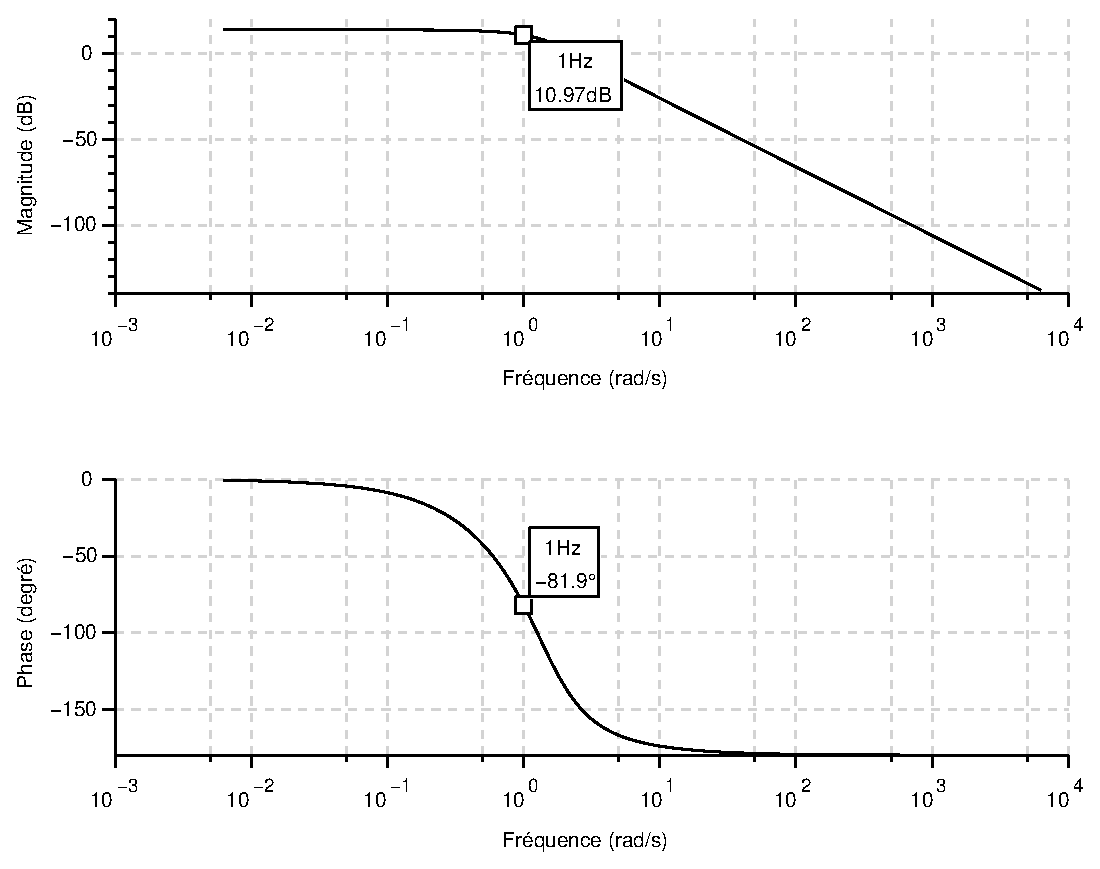
\includegraphics[width=0.75\textwidth]{bode_BONC_4.eps}
    \caption{Diagramme de Bode de la boucle ouverte non corrigée
             On a représenté le gain et la phase à la pulsation de coupure 
             $\omega_0=\SI{1}{\radian\per\second}$}
\end{figure}
%-------------------------------------------------------------------------------
%Q11
%%%%%%%%%%%%%%%%%%%%%%%%%%%%%%%%%%%%%%%%%%%%%%%%%%%%%%%%%%%%%%%%%%%%%%%%%%%%%%%%
\question{\textbf{Déterminer les paramètres $\tau_i$ et $K_i$ à partir des 
          relations du correcteur PI suivantes:}}
%%%%%%%%%%%%%%%%%%%%%%%%%%%%%%%%%%%%%%%%%%%%%%%%%%%%%%%%%%%%%%%%%%%%%%%%%%%%%%%%
%-------------------------------------------------------------------------------
\begin{align*}
    \tau_i=-\dfrac{1}{\omega_0\tan\phi_i}=\SI{1.27}{\second}\\
    K_i=\dfrac{G_i\tau_i\omega_0}{\sqrt{1+\tau^2_i\omega^2_0}}=0.222
\end{align*}
%-------------------------------------------------------------------------------
%Q12
%%%%%%%%%%%%%%%%%%%%%%%%%%%%%%%%%%%%%%%%%%%%%%%%%%%%%%%%%%%%%%%%%%%%%%%%%%%%%%%%
\question{\textbf{Donner la forme numérique de la fonction de transfert du 
          régulateur PI ainsi obtenu}}
%%%%%%%%%%%%%%%%%%%%%%%%%%%%%%%%%%%%%%%%%%%%%%%%%%%%%%%%%%%%%%%%%%%%%%%%%%%%%%%%
\[
    C_{PI}(p)=\dfrac{0.222 + 0.283p}{1.274p}
\]
%Q13
%%%%%%%%%%%%%%%%%%%%%%%%%%%%%%%%%%%%%%%%%%%%%%%%%%%%%%%%%%%%%%%%%%%%%%%%%%%%%%%%
\question{\textbf{Tracer le diagramme de Bode de la boucle ouverte corrigée 
          par ce correcteur}}
%%%%%%%%%%%%%%%%%%%%%%%%%%%%%%%%%%%%%%%%%%%%%%%%%%%%%%%%%%%%%%%%%%%%%%%%%%%%%%%%
%-------------------------------------------------------------------------------
\inputminted{scilab}{codes/scilab/code_q13_chap_correction.sce}
%-------------------------------------------------------------------------------
%-------------------------------------------------------------------------------
\begin{figure}
    \centering
    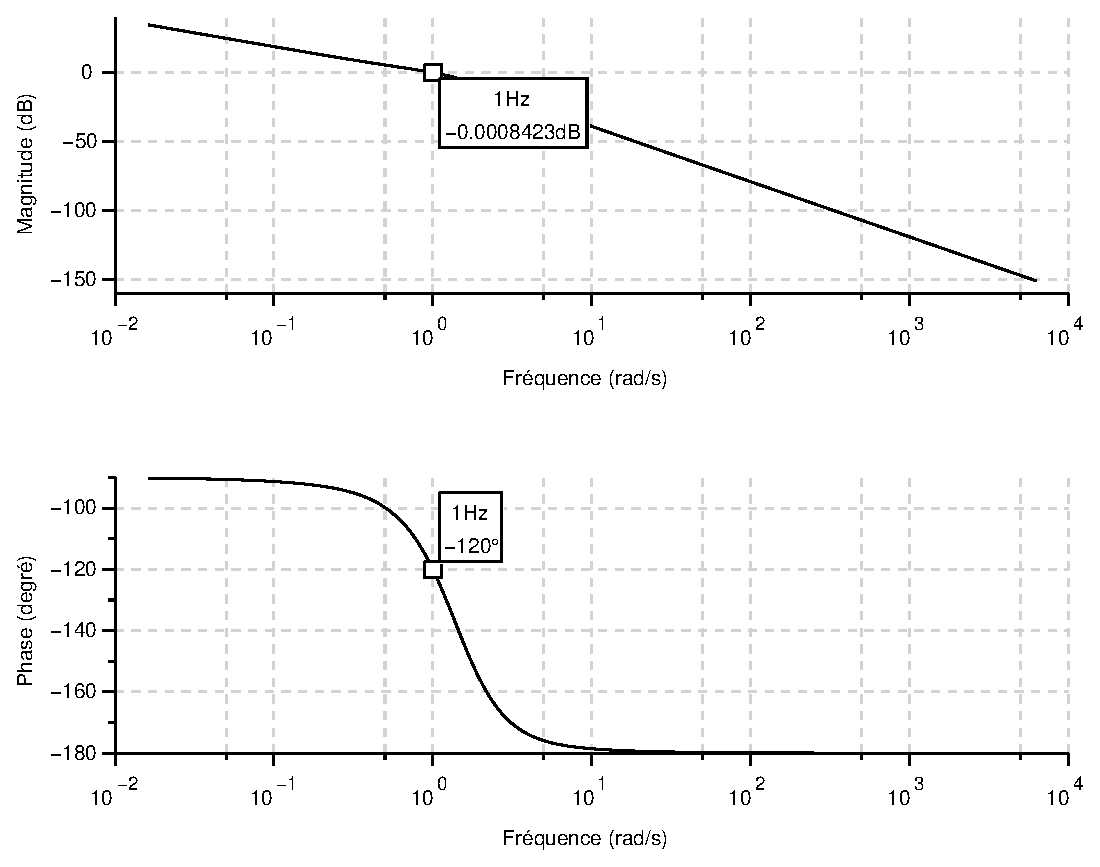
\includegraphics[width=0.75\textwidth]{bode_BOCPI.eps}
    \caption{Diagramme de Bode de la boucle ouverte corrigée par 
    le correcteur PI}
\end{figure}
%-------------------------------------------------------------------------------
On vérifie qu'à la pulsation de coupure le gain est nul (en \si{\dB}) et
que la phase donne une marge de phase de \SI{60}{\degreeSI}
%%%%%%%%%%%%%%%%%%%%%%%%%%%%%%%%%%%%%%%%%%%%%%%%%%%%%%%%%%%%%%%%%%%%%%%%%%%%%%%%
%%%%%%%%%%%%%%%%%%%%%%%%%%%%%%%%%%%%%%%%%%%%%%%%%%%%%%%%%%%%%%%%%%%%%%%%%%%%%%%%
\subsection*{Régulation du correcteur PID}
%%%%%%%%%%%%%%%%%%%%%%%%%%%%%%%%%%%%%%%%%%%%%%%%%%%%%%%%%%%%%%%%%%%%%%%%%%%%%%%%
%%%%%%%%%%%%%%%%%%%%%%%%%%%%%%%%%%%%%%%%%%%%%%%%%%%%%%%%%%%%%%%%%%%%%%%%%%%%%%%%
%Q14
%%%%%%%%%%%%%%%%%%%%%%%%%%%%%%%%%%%%%%%%%%%%%%%%%%%%%%%%%%%%%%%%%%%%%%%%%%%%%%%%
\question{\textbf{En utilisant la méthodologie précédente, déterminer les 
          paramètres des régulateurs composant ce PID}}
%%%%%%%%%%%%%%%%%%%%%%%%%%%%%%%%%%%%%%%%%%%%%%%%%%%%%%%%%%%%%%%%%%%%%%%%%%%%%%%%
La résolution du système de deux équations suivant:
\[
\begin{cases}
    \phi_d-\phi_i&=\SI{-180}{\degreeSI}+M_\phi-\arg{H(j\omega_0)} \\
    \phi_d+\phi_i&=\SI{90}{\degreeSI},
\end{cases}
\]
nous permet de déterminer numériquement les phases $\phi_d$ et 
$\phi_i$ des correcteurs. On obtient alors:
\[
\begin{cases}
    \phi_d=\SI{-45}{\degreeSI}+
           \dfrac{M_\phi-\arg{H(j\omega_0)}}{2}=\SI{66.39}{\degreeSI} \\
    \phi_i=\SI{135}{\degreeSI}+
           \dfrac{\arg{H(j\omega_0)}-M_\phi}{2}=\SI{23.61}{\degreeSI}
\end{cases}
\]

On a alors pour les paramètres des correcteurs :
%-------------------------------------------------------------------------------
\begin{itemize}
    \item[AP] 
%-------------------------------------------------------------------------------
        \begin{align*}
            \alpha&=22.89\\
            \tau_d&=\SI{0.052}{\second}\\
            K_d&=0.209
        \end{align*}
%-------------------------------------------------------------------------------
    \item[PI]
%-------------------------------------------------------------------------------
        \begin{align*}
            \tau_i&=\SI{0.572}{\second}\\
            k_i&=0.9163
        \end{align*}
%-------------------------------------------------------------------------------

\[
    k_p=2.97
\]
\end{itemize}
%-------------------------------------------------------------------------------
%Q15
%%%%%%%%%%%%%%%%%%%%%%%%%%%%%%%%%%%%%%%%%%%%%%%%%%%%%%%%%%%%%%%%%%%%%%%%%%%%%%%%
\question{\textbf{Donner la forme numérique de la fonction de transfert du 
          correcteur}}
%%%%%%%%%%%%%%%%%%%%%%%%%%%%%%%%%%%%%%%%%%%%%%%%%%%%%%%%%%%%%%%%%%%%%%%%%%%%%%%%
\[
    C_{AP}(p)=\dfrac{0.208 + 0.25p}{1+0.052p}
\]
\[
    C_{PI}(p)=\dfrac{0.916 + 0.524p}{0.572p}
\]
\[
    C_{PID}(p)=\dfrac{0.569+1.006p+0.389p^2}{0.572p+ 0.029p^2}  
\]
%Q16
%%%%%%%%%%%%%%%%%%%%%%%%%%%%%%%%%%%%%%%%%%%%%%%%%%%%%%%%%%%%%%%%%%%%%%%%%%%%%%%%
\question{\textbf{Tracer le diagramme de Bode de la boucle ouverte corrigée}}
%%%%%%%%%%%%%%%%%%%%%%%%%%%%%%%%%%%%%%%%%%%%%%%%%%%%%%%%%%%%%%%%%%%%%%%%%%%%%%%%
%-------------------------------------------------------------------------------
\inputminted{scilab}{codes/scilab/code_q16_chap_correction.sce}
%-------------------------------------------------------------------------------
%-------------------------------------------------------------------------------
\begin{figure}
    \centering
    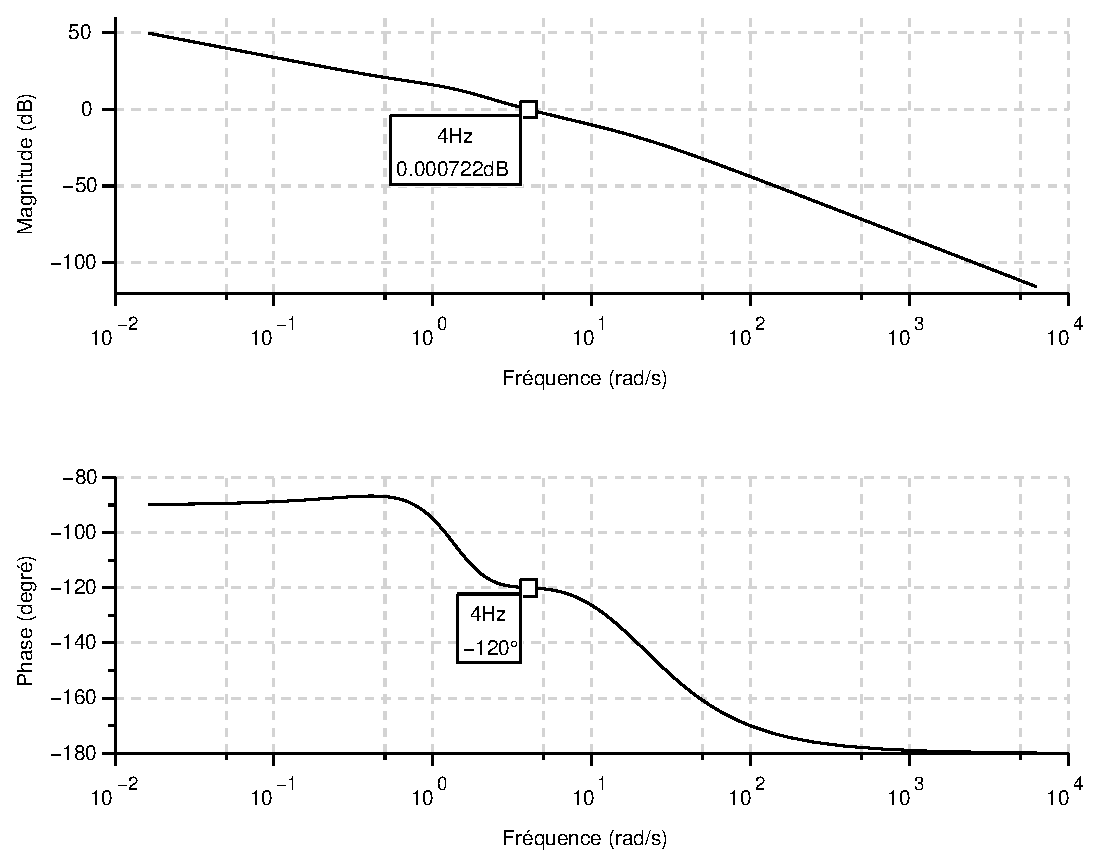
\includegraphics[width=0.75\textwidth]{bode_BOCPID.eps}
    \caption{Diagramme de Bode de la boucle ouverte corrigée par 
    le correcteur PID}
\end{figure}
%-------------------------------------------------------------------------------
On vérifie la phase et le gain à la pulsation de coupure.
%%%%%%%%%%%%%%%%%%%%%%%%%%%%%%%%%%%%%%%%%%%%%%%%%%%%%%%%%%%%%%%%%%%%%%%%%%%%%%%%
%%%%%%%%%%%%%%%%%%%%%%%%%%%%%%%%%%%%%%%%%%%%%%%%%%%%%%%%%%%%%%%%%%%%%%%%%%%%%%%%
\subsection*{Réponses temporelles en boucle fermée}
%%%%%%%%%%%%%%%%%%%%%%%%%%%%%%%%%%%%%%%%%%%%%%%%%%%%%%%%%%%%%%%%%%%%%%%%%%%%%%%%
%%%%%%%%%%%%%%%%%%%%%%%%%%%%%%%%%%%%%%%%%%%%%%%%%%%%%%%%%%%%%%%%%%%%%%%%%%%%%%%%
%Q17
%%%%%%%%%%%%%%%%%%%%%%%%%%%%%%%%%%%%%%%%%%%%%%%%%%%%%%%%%%%%%%%%%%%%%%%%%%%%%%%%
\question{\textbf{Comparer sur une figure les diagrammes de Bode de ces boucles 
          ouvertes corrigées et non corrigées}}
%%%%%%%%%%%%%%%%%%%%%%%%%%%%%%%%%%%%%%%%%%%%%%%%%%%%%%%%%%%%%%%%%%%%%%%%%%%%%%%%

%-------------------------------------------------------------------------------
\begin{figure}[!h]
    \centering
    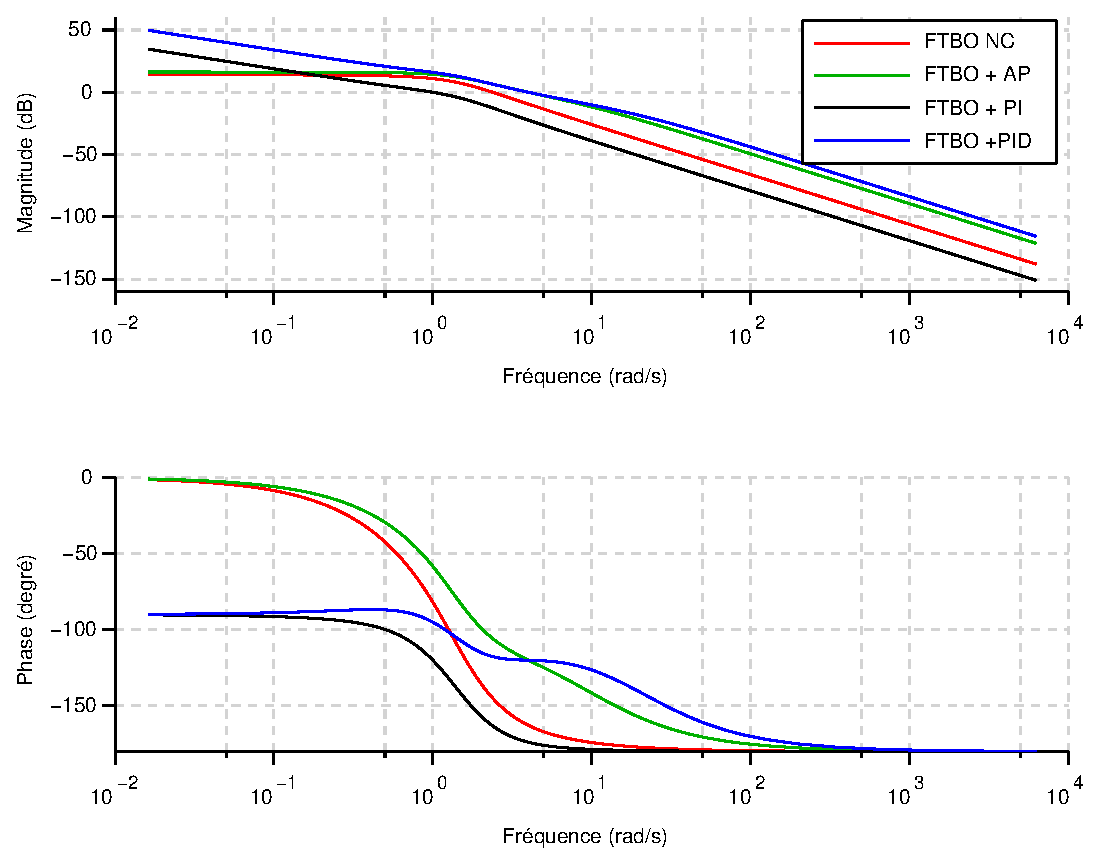
\includegraphics[width=0.75\textwidth]{bode_BOC_all.eps}
    \caption{Diagramme de Bode de la boucle ouverte corrigée par 
    le correcteur PID}
\end{figure}
%-------------------------------------------------------------------------------
\clearpage
%Q18
%%%%%%%%%%%%%%%%%%%%%%%%%%%%%%%%%%%%%%%%%%%%%%%%%%%%%%%%%%%%%%%%%%%%%%%%%%%%%%%%
\question{\textbf{Tracer les réponses indicielles en boucle fermée de tous ces 
          correcteurs. Conclure ses les performances corrigées.}}
%%%%%%%%%%%%%%%%%%%%%%%%%%%%%%%%%%%%%%%%%%%%%%%%%%%%%%%%%%%%%%%%%%%%%%%%%%%%%%%%
%-------------------------------------------------------------------------------
\begin{figure}
\centering
\tikzsetnextfilename
{reponse_indicielle_corrigee-exercices_corriges-chap_correction-ext}
\input{tikz/reponse_indicielle_corrigee-exercices_corriges-chap_correction.tex}
\caption{Réponse indicielle du système en boucle fermée non corrigé 
         et corrigé par les différents régulateurs 
         du TD.~\label{fig-reponses_indicielles}}
\end{figure}
%-------------------------------------------------------------------------------
On a tracé sur la même figure~\ref{fig-reponses_indicielles} en boucle fermée 
de tout les systèmes corrigés et non corrigés du TD. On observe clairement les
effets de chacun d'entre eux:
%-------------------------------------------------------------------------------
\begin{itemize}
%-------------------------------------------------------------------------------
    \item Avance de phase: 
%-------------------------------------------------------------------------------
        \begin{itemize}
            \item augmentation de la marge de stabilité 
                  (moins d'oscillations, réduction du déplacement)
            \item augmentation de la bande passante et donc de la rapidité
            \item le système n'est pas précis (elle augmente cependant par 
                  rapport au système non corrigé)
        \end{itemize}
%-------------------------------------------------------------------------------
    \item Proportionnel Intégral : 
%-------------------------------------------------------------------------------
        \begin{itemize}
            \item effet intégral : système précis et diminution de la rapidité 
        \end{itemize} 
%-------------------------------------------------------------------------------
    \item Proportionnel Intégral Dérivé :
%-------------------------------------------------------------------------------
        \begin{itemize}
            \item effet intégral : système précis
            \item effet dérivé : augmentation de la rapidité et 
                  diminution des oscillations.
        \end{itemize} 
%-------------------------------------------------------------------------------
\end{itemize}
%-------------------------------------------------------------------------------
\clearpage
%%%%%%%%%%%%%%%%%%%%%%%%%%%%%%%%%%%%%%%%%%%%%%%%%%%%%%%%%%%%%%%%%%%%%%%%%%%%%%%%
%%%%%%%%%%%%%%%%%%%%%%%%%%%%%%%%%%%%%%%%%%%%%%%%%%%%%%%%%%%%%%%%%%%%%%%%%%%%%%%%
\subsection*{Code Scilab complet}
%%%%%%%%%%%%%%%%%%%%%%%%%%%%%%%%%%%%%%%%%%%%%%%%%%%%%%%%%%%%%%%%%%%%%%%%%%%%%%%%
%%%%%%%%%%%%%%%%%%%%%%%%%%%%%%%%%%%%%%%%%%%%%%%%%%%%%%%%%%%%%%%%%%%%%%%%%%%%%%%%
%-------------------------------------------------------------------------------
\inputminted{scilab}{codes/scilab/code_exercice_chap_correction.sce}
%-------------------------------------------------------------------------------
